%!TEX root = ../../main.tex
\section{Extracting Intensities and Doses}
\label{sec:Extracting Intensities and Doses}
To perform the extrapolation it is necessary to know both the intensities of each observation of a reflection and the dose absorbed by the crystal at the time of the observation.
To extract the reflection intensity data, the diffraction images were integrated using MOSFLM as described in section \ref{sub:Data Processing}.
The data were then scaled using AIMLESS, but the $B$ factor correction was turned off to prevent correcting for overall radiation damage.
The reflection intensities were then output to an unmerged MTZ file and the data were read by running MTZDUMP and parsing the log.
Importantly each reflection intensity observation was stored along with its corresponding \textit{batch} (image) number, which would ultimately allow it to be assigned the correct dose.

To extract the correct DWD values, RADDOSE-3D was run with the corresponding experimental parameters as described in section \ref{sub:Data Collection and Dose Calculation}.
The difference is that rather than outputting one DWD value to represent the average DWD for all images in the dataset, the DWD values are obtained for each image.
To use the DWD with the dose dependent $\eta$ functions developed in chapter \ref{chap:Dose Decay Modelling}, the parameter values $B_0, \beta$ and $\gamma$ must be found.
However the method used to obtain the parameter values in section \ref{sub:Obtaining Model Parameter Values} requires the collection of multiple datasets, which may not be possible if the crystal is very radiation sensitive.
Thus a new method to obtain the parameter values was developed.

The idea is to exploit the fact that the volume element (voxel) of the crystal has its own relative diffraction efficiency.
The weighted average of the individual relative diffraction efficiencies will result in the observed relative intensity of the dataset.
Mathematically this is
\begin{equation}
    I_n/I_0 = \f{\int_{\bs{x}} RDE(D(\bs{x}); B_0, \beta, \gamma) \times F(\bs{x})\,\mathrm{d}\bs{x}}{\int_{\bs{x}} F(\bs{x})\,\mathrm{d}\bs{x}},
\end{equation}
where $I_n/I_0$ is the theoretical relative intensity value (note that the denominator is $I_0$ rather than $I_1$ as the extrapolation back to zero dose is the aim), $RDE$ is the RDE function given by equation \ref{eqrdeleal}, $D$ is the absorbed dose, $F$ is the fluence and the vector $\bs{x}$ is the position in the crystal.
The absorbed dose and fluence for each voxel is returned in a file output by RADDOSE-3D representing the dose state of the crystal.
The parameters can then be found using an optimisation routine to minimise the squared residual between $I_n/I_0$ and $I_n/I_1$, where $I_n/I_1$ represent the measured relative intensities.
Matlab's \verb+lsqnonlin+ function was used for the optimisation, which in turn uses the trust-region-reflective algorithm \cite{coleman1996} or the Levenberg-Marquardt algorithm \cite{more1978levenberg} if the number of relative intensity measurements is less than the number of parameters.
Further to being able to fit the decay parameters for a single dataset, this method is able to deal with fitting parameters from inhomogeneous dose distributions.
An example case where ten 90$^{\circ}$ wedge datasets from crystal 0259 was used, the parameter values obtained are: $B_0 = 14.28\,\text{\AA}^2, \beta = 0.510\,\text{\AA}^2 \text{MGy}^{\text{-1}}$ and $\gamma = 0.047\,\text{MGy}^{\text{-1}}$, which are comparable to the values given in Table \ref{tab:RDE params1}.
The resulting $RDE$ is plotted in Figure~\ref{fig:Relative diffraction efficiency plot - ZDE}.
\begin{figure}
  \centering
    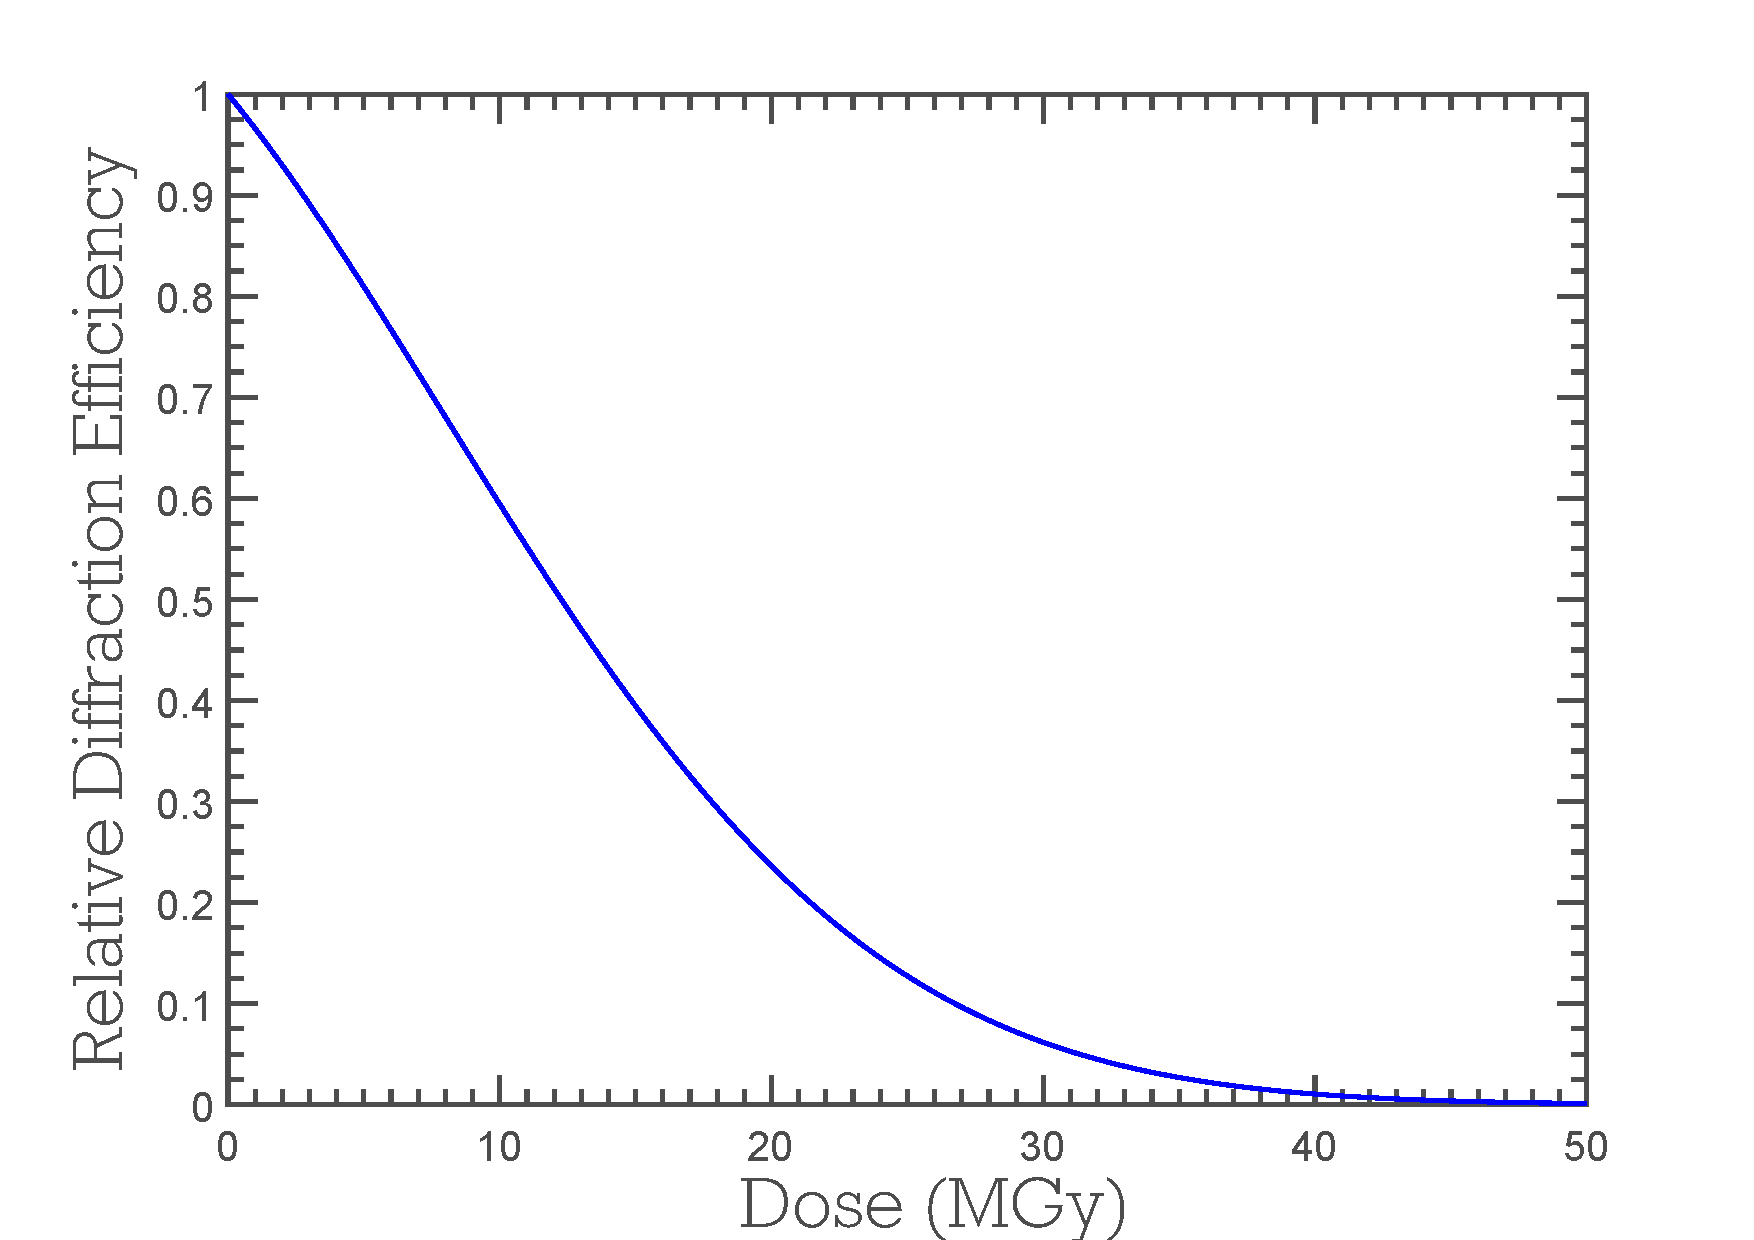
\includegraphics[width=1\textwidth]{figures/zde/RDEPlot_zde.pdf}
    \caption[Relative diffraction efficiency as a function of the dose.]{Relative diffraction efficiency plot with parameter values $B_0 = 14.28\,\text{\AA}^2, \beta = 0.510\,\text{\AA}^2 \text{MGy}^{\text{-1}}$ and $\gamma = 0.047\,\text{MGy}^{\text{-1}}$.}
    \label{fig:Relative diffraction efficiency plot - ZDE}
\end{figure}

One obvious issue with only using a single dataset for this optimisation is that $I_n/I_1 = 1$ for the first dataset by definition, whereas $RDE(D)$ is less than 1 for any dose greater than zero.
To circumvent this issue, the observed relative intensity data are scaled to more accurately represent the relative intensity with respect to the theoretical zero-dose, $I_0$, prior to the parameter optimisation.
To scale the data, the following function was first fitted to the data
\begin{equation}
    I_n/I_0(D) = k e^{aD^2 + bD},
    \label{eq:Relative intensity scaling - resolution independent Leal model}
\end{equation}
where $k, a$ and $b$ are parameters to be determined.
A closer inspection shows that this equation is a more general form of the Leal \textit{et al.} model where the resolution dependence has been omitted.
The dose metric used here is the simple DWD (equation \ref{eq:DWD equation - no RDE}), because at this point there is no information about the parameter values required to calculate $\eta$.
For small dose ranges, the simple DWD is a suitable approximation for the DWD with dose dependent $\eta$ terms, because for small doses, $\eta(D) \approx 1$.
A least squares curve fitting procedure, Matlab's \verb+lsqcurvefit+ routine, was used to fit the relative intensity data to the function defined in equation \ref{eq:Relative intensity scaling - resolution independent Leal model}.
The relative intensity data were then scaled by $k$.
The result of the relative intensity scaling for the example above (ten 90$^{\circ}$ wedge datasets from crystal 0259) is shown in Figure~\ref{fig:Scaled relative intensity data - ZDE}.
\begin{figure}
  \centering
    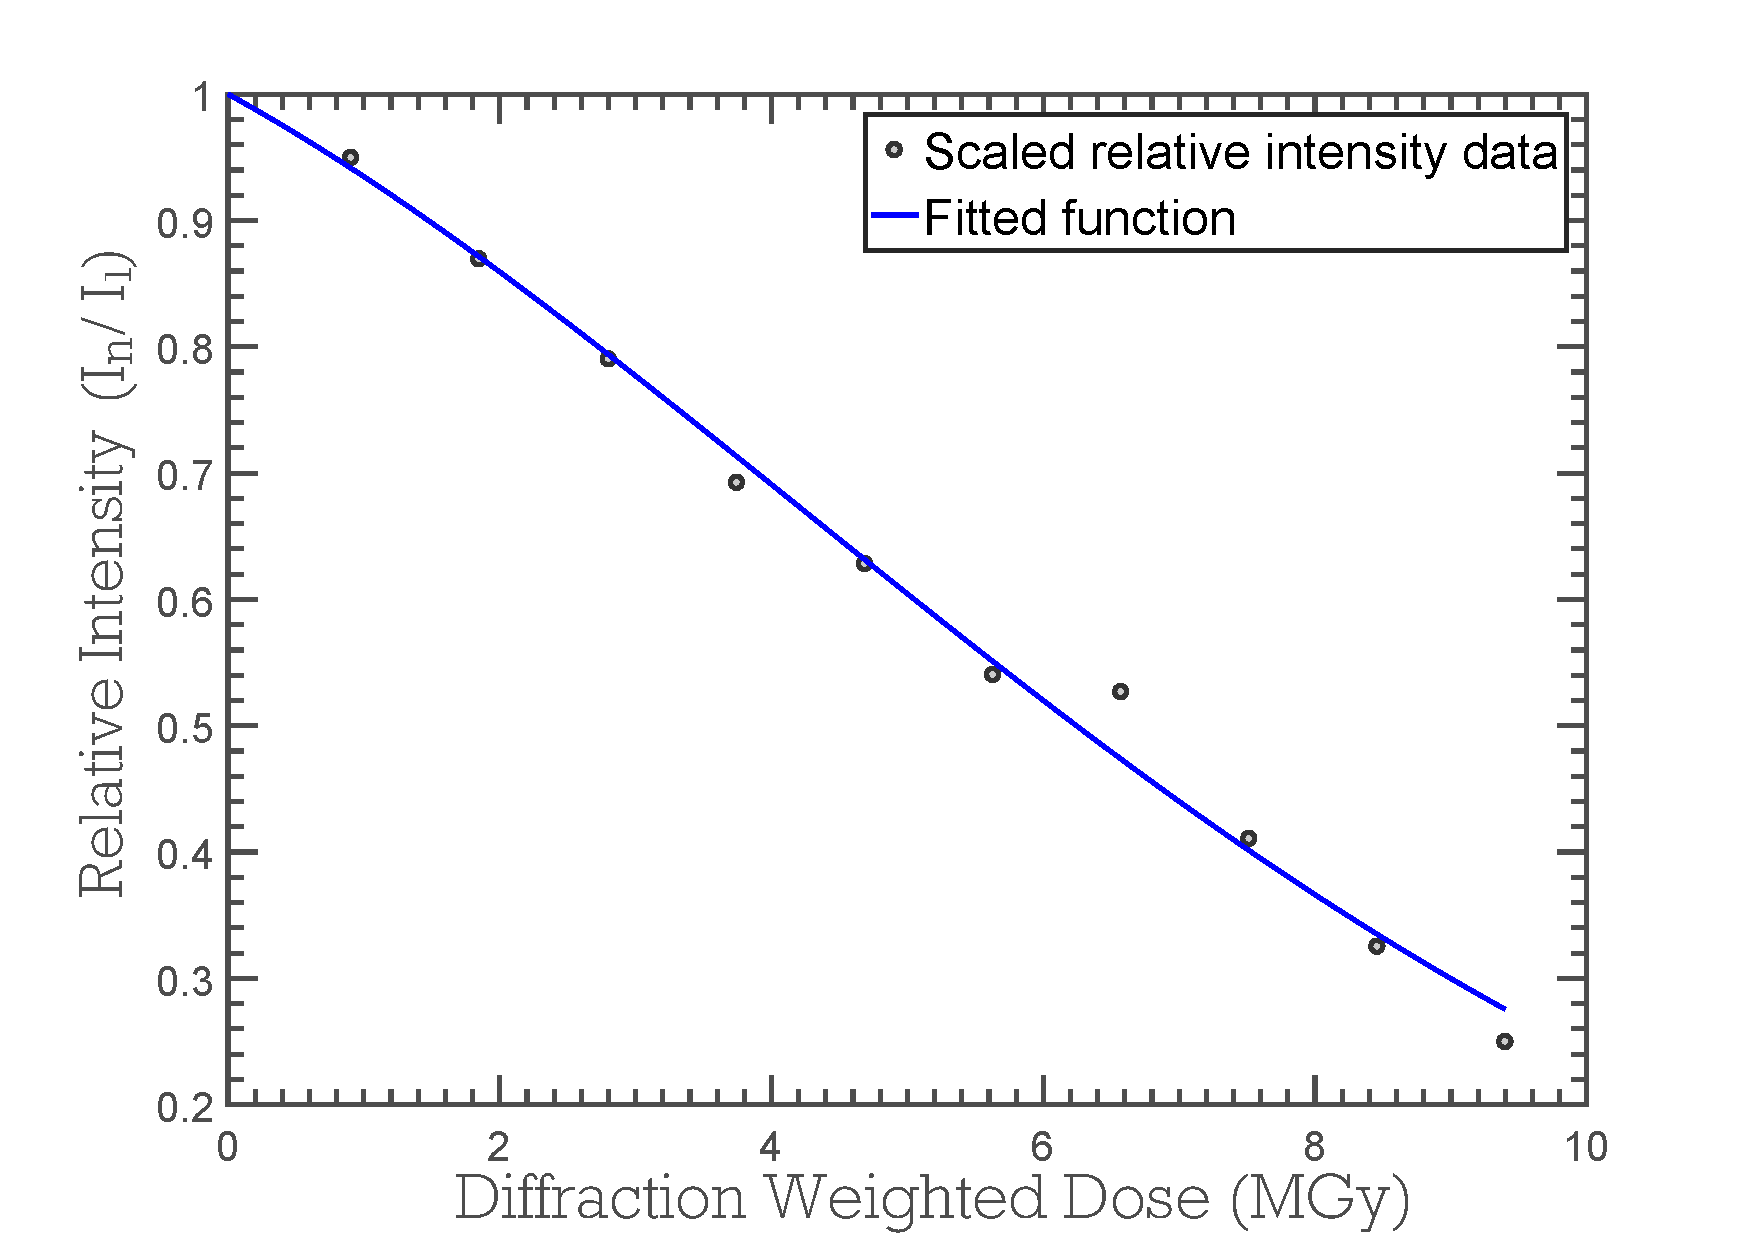
\includegraphics[width=1\textwidth]{figures/zde/ScaledFunctionFitPlot.pdf}
    \caption[Scaled relative intensity decay.]{Scaled relative intensity data (grey circles) for cubic insulin crystal (crystal ID 0259) plotted with the fitted function (equation \ref{eq:Relative intensity scaling - resolution independent Leal model}) overlaid.}
    \label{fig:Scaled relative intensity data - ZDE}
\end{figure}
